\documentclass{article}
\usepackage{graphicx}
\usepackage{hyperref}
\usepackage{amsmath}
\usepackage{enumitem}

\title{LLM Anonymization Techniques Recommender for Datasets (LLMANO-2)}
\author{Amin Akziz, Leander Ziehm, Azba Engineer, Santiago}
\date{April 2025}

\usepackage[a4paper, margin=1in]{geometry}

\usepackage{setspace}
\onehalfspacing

\begin{document}

\maketitle

\begin{center}
\begin{minipage}{0.85\textwidth}
\section*{Abstract}
The need for anonymizing datasets has grown significantly with the proliferation of machine learning and large language models (LLMs). However, many users lack a clear understanding of how to properly anonymize their data without significantly compromising its utility. In response to this challenge, we present LLMANO-2, a recommender system that leverages LLMs to guide users in anonymizing CSV datasets while preserving predictive performance. Our system provides tailored recommendations based on the specific characteristics of each dataset, aiming to strike a balance between privacy and usability. The motivation for this work stems from recent data privacy incidents that highlight the risks of improper anonymization and the growing demand for practical, intelligent tools to support privacy-aware data publishing.
\end{minipage}
\end{center}

\section{Introduction}

In today’s era of big data and artificial intelligence, vast amounts of personal and sensitive information are being collected and analyzed. This proliferation of data has made dataset anonymization a critical concern, as organizations must protect individual privacy while still deriving value from the data. 

A dataset (for example, a CSV file or database table) typically consists of many records (rows) with multiple attributes (columns) describing each record. These attributes can include direct identifiers (such as names, email addresses, or national ID numbers) as well as indirect identifiers (such as dates of birth, gender, or ZIP codes) that might not identify someone on their own, but could do so when combined with other information.

Data anonymization refers to the process of modifying a dataset to remove or obscure personal identifiers so that individuals cannot be readily identified. In essence, it involves “erasing or encrypting identifiers that connect an individual to stored data,” while ideally retaining the data’s overall usefulness. The goal is to strike a balance between privacy and utility, ensuring that the data remains valuable for analysis or machine learning, but that it no longer reveals private information about individuals.

In practice, anonymization techniques may include removing or masking direct personal identifiers, generalizing values (for example, replacing an exact age with an age range), or pseudonymizing data by replacing real identifiers with artificial codes apart from other techniques. By transforming personal data into a format that cannot be linked to specific individuals, anonymization ensures privacy while allowing organizations to leverage the data for insights.

\begin{figure}[h]
    \centering
    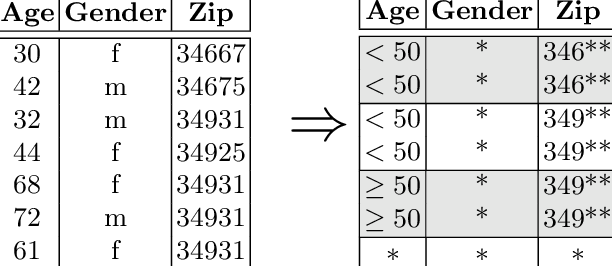
\includegraphics[width=0.65\linewidth]{images/figure1.png}
    \caption{Example of an anonymization technique applied to a simple dataset}
    \label{fig:anonymization-example}
\end{figure}


This is especially important when sharing datasets with third parties or releasing them publicly for research, as it enables data sharing and collaboration without compromising the confidentiality of the people described by the data. Notably, data anonymization is not just a best practice but often a legal requirement: privacy regulations like the EU’s General Data Protection Regulation (GDPR) and the California Consumer Privacy Act (CCPA) mandate that personal data be anonymized or otherwise protected if it’s to be used beyond its original purpose. Failure to properly anonymize data can lead to severe regulatory penalties as well as loss of user trust.

Despite its importance, effective anonymization can be challenging, and previous evidence has shown that improperly anonymized datasets can still compromise privacy. Certain data attributes are extremely sensitive, and even “anonymized” data can be re-identified by clever attackers. A famous statistic by Latanya Sweeney demonstrated that 87\% of the U.S. population could be uniquely identified using only three pieces of information – birth date, gender, and ZIP code – highlighting how a few quasi-identifiers combined together can pinpoint individual.

Another example where personal data was compromised is in the Netflix Prize dataset released in 2006, which contained movie ratings with personal identities removed, researchers were able to re-identify specific users by correlating the anonymized ratings with public information on IMDb (Internet Movie Database). This meant that personal viewing preferences (and even sensitive attributes inferred from them) of certain Netflix users became public, despite Netflix’s attempt to anonymize the data.

These cases underscore that simply removing obvious identifiers is often not sufficient, if enough data remains, determined adversaries can link supposedly anonymous records back to real individuals. Beyond the harm to individuals (exposing someone’s health information, financial status, location history, etc.), such incidents also expose organizations to legal liabilities and reputational damage. As data mining and cross-referencing techniques grow more sophisticated in today’s “big data” age, re-identification attacks are becoming easier and more common. This puts pressure on data publishers to adopt stronger anonymization measures than were needed in the past.

At the same time, data anonymization must be done carefully to preserve the usefulness of data. Over-aggressive anonymization (for instance, deleting or randomizing too many fields) can render a dataset nearly useless for analysis or model training, defeating the purpose of sharing the data in the first place. There is an inherent trade-off between privacy and utility: the more information we strip away or distort to protect privacy, the less accurate or insightful the dataset becomes. A core challenge is finding the sweet spot where sensitive personal details are well-protected, yet the anonymized dataset still supports meaningful insights or predictions. Achieving this balance often requires expertise and context, deciding which attributes can be generalized or masked, and to what extent, without overly degrading the data’s integrity. Unfortunately, many users and organizations lack a clear understanding of how to properly anonymize their data to meet this balance. Choosing the right anonymization techniques is not trivial: it depends on the data content, the presence of auxiliary data that attackers might use, and the intended use of the anonymized data. As a result, there is a growing need for tools and guidance to help data owners to navigate this complexity.

Recently, advances in Artificial Intelligence have introduced new possibilities for smarter anonymization approaches. In particular, Large Language Models (LLMs) offer a promising idea to tackle the privacy-utility trade-off. In alignment with these developments, our work proposes LLMANO-2, an LLM-powered anonymization technique based recommender for datasets. LLMANO-2 is designed to assist users in anonymizing tabular datasets by recommending appropriate techniques for each column of data. For a given dataset, the system leverages an LLM to analyze the column contents and identify which fields are likely sensitive and suggest how to transform or mask them. The recommendations aim to maximize privacy protection while minimizing the impact on the dataset’s utility for analysis or machine learning tasks. In the following sections we describe the architecture and methodology behind LLMANO-2, including how it processes datasets, generates anonymization recommendations, and evaluates the effectiveness of those recommendations.



\section{Background/Theory}
We outline key privacy concepts including:
\begin{itemize}
    \item \textbf{Direct identifiers} (e.g., names, emails)
    \item \textbf{Quasi-identifiers} (e.g., weight, height, age)
    \item \textbf{Anonymity metrics} such as $k$-Anonymity and $l$-Diversity, t-closeness
    \item \textbf{Anonymization Methods}
\end{itemize}
We also introduce user-driven anonymization processes and the limitations of manual or rule-based methods.

In this section, we outline the mathematical foundations underlying key privacy-preserving techniques in data publishing, namely $k$-anonymity, $l$-diversity, and generalization strategies.

\subsection{Identifiers and Quasi-Identifiers}

In the context of privacy-preserving data analysis, it is essential to distinguish between different types of attributes:

\begin{itemize}
\item \textbf{Direct Identifiers} are attributes that can uniquely identify an individual without external information. Common examples include names, social security numbers, or email addresses.

\item \textbf{Indirect Identifiers}, also called \textit{quasi-identifiers}, are attributes that do not uniquely identify an individual on their own but can do so when combined with other quasi-identifiers. Examples include age, ZIP code, and gender.
\end{itemize}

Effective anonymization techniques aim to remove or transform these identifiers such that the risk of re-identification is minimized.

\subsection{$k$-Anonymity}

The concept of $k$-anonymity, introduced by Sweeney, is one of the foundational principles for privacy protection. A dataset is said to satisfy \textbf{$k$-anonymity} if each record is indistinguishable from at least $k-1$ other records with respect to the quasi-identifiers.

Formally, given a dataset $D$ with quasi-identifier attributes $Q_1, Q_2, ..., Q_m$, let $\pi$ be a projection onto the quasi-identifier space:

$$
\pi(D) = \{ (q_1, q_2, ..., q_m) \mid (q_1, ..., q_m) \in D \}
$$

Let $E$ be an equivalence class of records in $D$ that share the same quasi-identifier values:

$$
E = \{ r \in D \mid \forall i, \; r[Q_i] = v_i \}
$$

Then $D$ satisfies $k$-anonymity if:

$$
\forall E \subseteq D, \quad |E| \geq k
$$

This ensures that an adversary cannot link any given record to fewer than $k$ individuals. However, $k$-anonymity alone does not prevent \textit{attribute disclosure}—when sensitive values within a group are too homogeneous.

\subsection{$l$-Diversity}

To address the limitations of $k$-anonymity, the notion of \textbf{$l$-diversity} was proposed. It enhances privacy by requiring that each equivalence class (i.e., group of records sharing the same quasi-identifiers) contains at least $l$ "well-represented" values for the sensitive attribute.

Mathematically, let $S$ be the sensitive attribute. An equivalence class $E$ satisfies \textit{distinct $l$-diversity} if:

$$
|\{ r[S] \mid r \in E \}| \geq l
$$

This means that in each equivalence class, there are at least $l$ distinct values for the sensitive attribute.

More robust variants include:
\begin{itemize}
\item \textbf{Entropy $l$-Diversity}, which requires the entropy of the sensitive attribute distribution in each class to be at least $\log l$:
$$
-\sum_{s \in S} p_s \log p_s \geq \log l
$$
where $p_s$ is the fraction of records in the class with sensitive value $s$.

\item \textbf{Recursive (c, $l$)-Diversity}, which prevents skewness by limiting how dominant the most frequent sensitive value can be.
\end{itemize}

\subsection{Anonymization Methods}
We summarize several key anonymization techniques, each suited to different data contexts and privacy requirements.

\textbf{Suppression} involves fully removing specific cells or rows from a dataset. It is most suitable for quick removal of extremely sensitive data, especially in open-data publication settings.

\textbf{Generalization} clusters records and replaces each cluster with a representative centroid or more general category. This method is particularly effective for numerical data and statistical summaries and supports privacy models such as $k$-Anonymity and $l$-Diversity. It is often used when preparing datasets for open-data release.

\textbf{Differential Privacy (Global, DP-SGD)} relies on query-based data release mechanisms where calibrated noise is added to the output. It is best suited for machine learning training (e.g., with DP-SGD) and interactive analytics, where a defined privacy budget (e.g., epsilon, delta) must be managed.

\textbf{Differential Privacy (Local)} applies privacy-preserving noise at the individual data record level before data collection. This method is ideal for decentralized or mobile data gathering scenarios, such as collaborative research with privacy guarantees at the point of data generation.

\textbf{Pseudonymization} replaces identifiers with consistent tokens, allowing data to remain linkable while obscuring personally identifiable information. It is often applied for regulatory compliance purposes.

\textbf{Tokenization} substitutes identifiers with cryptographic tokens and may leverage secure multiparty computation techniques. It enables privacy-preserving collaborative analysis and is well-suited for research collaboration contexts.

In addition to these methods, \textbf{homomorphic encryption} offers another avenue for privacy-preserving computation, allowing data to be processed while still encrypted. This enables secure computation without ever revealing the underlying sensitive values.

AGAIN CAN DELETE: Generalization

Achieving $k$-anonymity and $l$-diversity typically requires generalization and/or suppression of quasi-identifier attributes. Generalization replaces specific values with broader categories. For example:
\begin{itemize}
\item Age: 23 $\rightarrow$ [21--30]
\item ZIP Code: 12345 $\rightarrow$ 123**
\end{itemize}
more here todo leander. 


The goal is to form equivalence classes with sufficient cardinality and sensitive attribute diversity, while minimizing information loss.





\section{Architecture}
\begin{itemize}
    \item Setup and hardware needed
    \item Overview diagram of system components
    \item LLM interface and decision flow
    \item Form interface for user inputs (direct/quasi identifier tagging)
    \item Backend anonymization and evaluation pipeline
\end{itemize}

\section{Related Work}
This section reviews:
\begin{itemize}
     \item The paper where we got the from from
     \item Risk analysis papers
    \item LLM-based anonymization

\end{itemize}
We discuss the differences in our approach, emphasizing interactive recommendation and fine-grained generalization control.

\section{Evaluation}
Our system allows users to:
\begin{enumerate}
    \item Upload CSV datasets
    \item Select columns as direct or quasi-identifiers (form includes definitions and examples)
    \item Receive LLM-generated anonymization recommendations (e.g., $k=10$)
    \item Optionally adjust granularity and generalization steps
\end{enumerate}
LLMs are prompted to recommend anonymization strategies based on dataset structure and user inputs. Screenshots and/or GitHub links will be included.

We test our system on multiple datasets:
\begin{itemize}
    \item Comparison against human-created anonymization
    \item Benchmarking against other anonymization algorithms
    \item Metrics: preservation of predictive accuracy, anonymity scores
\end{itemize}
Each configuration is tested 10 times to compute average performance. Evaluation is automated and requires no user interaction.

\section{Limitations, Discussion, and Future Work}
\begin{itemize}
    \item Current setup lacks real-time chat interaction for refinement
    \item Scope limited to $k$-Anonymity and $l$-Diversity and t-closeness; future integration of differential privacy
    \item Broader comparison with more anonymization techniques needed
    \item Challenges in dataset diversity and granularity recommendation
\end{itemize}

\section{Conclusion}
We presented a prototype LLM-powered anonymization recommender that assists users in balancing privacy with data utility. Our system enables informed anonymization decisions and shows promise compared to existing approaches. Future enhancements will include conversational interfaces and broader evaluation.


\begin{thebibliography}{9}

\bibitem{li2018}
N.~Li \emph{et~al.},
“On sampling, anonymization, and differential privacy…,”
\emph{IEEE Trans.\ Knowledge and Data Engineering}, 2018.
\href{https://www.tandfonline.com/doi/full/10.1080/17579961.2018.1452176#abstract}{%
\texttt{doi:10.1080/17579961.2018.1452176}
}

\bibitem{esser2023}
E.~Esser \emph{et~al.},
“Privacy attacks on LLMs and how to defend,”
\emph{Science Advances}, 2023.
\href{https://www.science.org/doi/full/10.1126/sciadv.adn7053}{%
\texttt{doi:10.1126/sciadv.adn7053}
}

\bibitem{fake_news_dataset}
Clément Bisaillon, 
\emph{Fake and Real News Dataset}. Kaggle. 
\href{https://www.kaggle.com/datasets/clmentbisaillon/fake-and-real-news-dataset}{https://www.kaggle.com/datasets/clmentbisaillon/fake-and-real-news-dataset}

\bibitem{lending_club_dataset}
Wordsforthewise, 
\emph{Lending Club Dataset}. Kaggle. 
\href{https://www.kaggle.com/datasets/wordsforthewise/lending-club/data}{https://www.kaggle.com/datasets/wordsforthewise/lending-club/data}

\bibitem{student_demographics_dataset}
Anıl Gürbüz, 
\emph{Student Demographics – Online Education Dataset}. Kaggle. 
\href{https://www.kaggle.com/datasets/anlgrbz/student-demographics-online-education-dataoulad}{https://www.kaggle.com/datasets/anlgrbz/student-demographics-online-education-dataoulad}

\bibitem{hospital_discharges_dataset}
Bhautik Mangukiya, 
\emph{Hospital Inpatient Discharges Dataset}. Kaggle. 
\href{https://www.kaggle.com/datasets/bhautikmangukiya12/hospital-inpatient-discharges-dataset}{https://www.kaggle.com/datasets/bhautikmangukiya12/hospital-inpatient-discharges-dataset}

\bibitem{adult_income_dataset}
UCI Machine Learning Repository, 
\emph{Adult Census Income Dataset}. Kaggle. 
\href{https://www.kaggle.com/datasets/uciml/adult-census-income/data}{https://www.kaggle.com/datasets/uciml/adult-census-income/data}

\bibitem{titanic_dataset}
Yasser Hatab, 
\emph{Titanic Dataset}. Kaggle. 
\href{https://www.kaggle.com/datasets/yasserh/titanic-dataset}{https://www.kaggle.com/datasets/yasserh/titanic-dataset}


\end{thebibliography}
\end{document}
